\documentclass[12pt]{article}

\usepackage{hyperref}
\hypersetup{
	colorlinks,
	citecolor=blue,
	%filecolor=black,
	linkcolor=black,
	urlcolor=blue
}
\usepackage{float}
\usepackage[english]{babel}
\usepackage[square,numbers]{natbib}
\bibliographystyle{abbrvnat}
\usepackage{url}
\usepackage[utf8x]{inputenc}
\usepackage{amsmath}
\usepackage{graphicx}
\graphicspath{{images/}}
\usepackage{parskip}
\usepackage{fancyhdr}
\usepackage{vmargin}
\PassOptionsToPackage{hyphens}{url}\usepackage{hyperref}
\setmarginsrb{3 cm}{2.5 cm}{3 cm}{2.5 cm}{1 cm}{1.5 cm}{1 cm}{1.5 cm}
\usepackage[table]{xcolor}
\usepackage{todonotes}
\usepackage{menukeys}

\title{Spatiotemporal Data Classification}   % Title
\author{ Nikiforos Pittaras, M1422 \\ 
		 Chrysoula Themeli, M1423}                               % Authors
\date{\today}  % Date

\makeatletter
\let\thetitle\@title
\let\theauthor\@author
\let\thedate\@date
\makeatother

\pagestyle{fancy}
\fancyhf{}
%\rhead{\theauthor}
\lhead{\thetitle}
\cfoot{\thepage}

\begin{document}
	
	%%%%%%%%%%%%%%%%%%%%%%%%%%%%%%%%%%%%%%%%%%%%%%%%%%%%%%%%%%%%%%%%%%%%%%%%%%%%%%%%%%%%%%%%%
	
	\begin{titlepage}
		\centering
		\vspace*{0.5 cm}
		
\includegraphics[scale = 0.75]{ekpalogo.png}\\[1.0 cm]   % University Logo
		\textsc{\LARGE National and Kapodistrian University of Athens}\\[2.0 cm]   % University Name
		\textsc{\Large Department of Informatics and Telecommunications}\\[0.5 cm]               % Department
		\textsc{\large Large-Scale Data Analysis Techniques}\\[0.5 cm] % Course Name
		\rule{\linewidth}{0.2 mm} \\[0.4 cm]
		{ \huge \bfseries \thetitle}\\
		\rule{\linewidth}{0.2 mm} \\[1.5 cm]
		
		\begin{minipage}{0.4\textwidth}
			\begin{center} \large
				\theauthor
			\end{center}
		\end{minipage}~
		\begin{minipage}{0.4\textwidth}
		\end{minipage}\\[2 cm]
		
		{\large \thedate}\\[2 cm]
		
		\vfill
		
	\end{titlepage}
	
	%%%%%%%%%%%%%%%%%%%%%%%%%%%%%%%%%%%%%%%%%%%%%%%%%%%%%%%%%%%%%%%%%%%%%%%%%%%%%%%%%%%%%%%%%
	
	\tableofcontents
    \newpage
	\listoffigures
	\newpage
	\listoftodos
	\newpage
	
	%%%%%%%%%%%%%%%%%%%%%%%%%%%%%%%%%%%%%%%%%%%%%%%%%%%%%%%%%%%%%%%%%%%%%%%%%%%%%%%%%%%%%%%%%

	\section{Introduction}
    This is the report related to the Python project for the course "Large-Scale Data Analysis Techniques". In the below sections, the implemented logic will be explicitly analyzed. The project is divided in two parts: in the first part the goals are: to preprocess and clean the given data as well as to visualize five of the given trips in the train\_set file. In the second part, the tasks are: to find for all test trips the k nearest neighbors from the given train trips, to find the train trips with the longest similar sub-route for each test trip, to use 10-fold cross validation to the training data and classify them with three different methods (k-nearest neighbors, logistic regression and random forest), to choose one of the above classification methods and improve the result and finally to test the classifier on some given test data.
    
    In the main.py file, it is required to provide the path to the input folder (containing the training and test files) and the output folder where all results will be stored. Afterwards, an object containing all the necessary for the program options is created. This object includes options such as the given input and output directories, the train and the required test files, the number of cells in the grid to be constructed, the number of nearest neighbors etc. There are two ways in order to run this project, either add these folders in the edit configurations choice from the menu, or use the run.sh in order to provide these args. Finally, the dependencies are checked and the folders and files are prepared before starting to run the application.
    
	\section{Exercise 1}
	In this section, further details are provided related to the preprocessing and cleaning of the training data as well as to the trip's visualization. All files implementing the requirements of this part are in the file question1.py.
	
	\subsection{Data Preprocessing (question A)}
	The requirement in this part is to preprocess the input training data and create a new file with 3 columns, containing the trip\_id (a number incrementing by 1 for each trip), the journey\_id(excluding trips with null id) and all points and timestamps in the format: [[timestamp1, longitude1, latitude1], [timestamp2, longitude2, latitude2],...]. The given csv file with the training data was transformed to a dataframe using the pandas library. The data with null journeyPatternId should be removed from the dataframe, therefore the lines are checked for NaN and "null" journey id. Then, the columns vehicleID and journeyPatternId are groupedby three times in order to create three different dataframes. For example, the first dataframe contains the columns: vehicleID, journeyPatternId and timpestamp. In a similar way, the two remaining dataframes were formatted. By concatenating them, the final dataframe contains five columns, where the three last columns contain a list of timestamps, a list of longitudes and a list of latitudes respectively.
	
	By iterating to each dataframe's row, the three lists are now concatenated in one column and therefore the other two are dropped from the dataframe. Then, the column vehicleID is replaced by the tripId column which is the index of this dataframe, starting from 0 and incrementing by 1. Finally, the column points, which now contains the list of lists with the timestamps and the points, is sorted based on the timestamp of each list item. The final result is exported in a file with the requested format.
	
	\subsection{Clean Data (question B)}
	The second goal was to clean the given data, based on two criteria: total trip distance should not be less than 2km while max distance between two successive points should not exceed 2km.
	
	The above logic is implemented in function filter\_trips. The two lists (trips\_too\_small and trips\_too\_big) will keep the excluded trips due to either not valid total distance or to invalid max distance between successive points. For each trip in the training dataset the total distance is calculated, using the function calculate\_lonlat\_distance, which returns the distance between two successive points using the haversine formula. Following the same logic, the max distance between successive points of a trip is calculated and a distance is found more than 2km, the trip is excluded.
	
	Finally, the distances are checked and rows with invalid trips are removed from the dataframe, which is, afterwards, exported in a new file (trips\_clean.csv).
	
	\subsection{Trip Visualization (question C)}
	This task is implemented in the function visualize\_trips and the created output is stored in the output folder in the gmplots directory. The requirement is to visualize five of the given train trips. For this purporse, the trips list is shuffled in order to visualize random trips and then iterated only for 5 trips. Then, a points list is created having two tuples with all the longitudes and latitudes(function idx\_to\_lonlat in the utils.py). 
	
	Finally, the function write\_group\_gml from the utils.py file is called. In this function, it is calculated the mean for both longitudes and latitudes and then gmplot is used so as to visualize the selected trips. Below, there is an example of a trip shown on map is presented:
	
	\begin{figure} [H]
		\begin{center}
			
\includegraphics [scale = 0.75] {questionCexample.jpg}
			\caption{Example of trip visualization}
		\end{center}
	\end{figure} 
	
	\section{Exercise 2}
	The files implementing the requirements of this part are in the file question2.py and some functions implementing the logic for this question are in the files: NearestNeighbors.py, NearestSubroutes.py, MapInGridView, JourneyClassification.py.
	
	\subsection{Nearest Neighbors (question A1)}
	For this part a test file is given (test\_set\_a1.csv, included in the input folder) containing additional trips. For each of these trips, the k nearest neighbors are targeted (in this exercise k=5) and an image file is produced, showing all six trips (the test trip and the trips from the training file) on six different maps. Under each map, the test or neighbor index, the journey\_id, the dynamic time warping and the time needed to process the neighbors of this test trip in millisecond.
	
	In the function question\_a1, two dataframes are created for both the test and the training trips. The test dataframe's rows are iterated and for each row the function calculate\_nns from the file NearestNeighbors.py is called in order to get the nearest neighbors, calculating also the time needed for this action.
	
	There are three ways to execute this task: using processes, threads or serial execution. This information is provided as input giving the kind of execution and the number of processes/threads as well. In the function run\_with\_processes an async task is executed for each process and then the result is stored in a list, while in the function run\_with\_threads, the dataframe is splitted in sub dataframes (the number is specified by the number of threads) and then distance is calculated for each subdataframe. After thread join, the result is also stored in the nearest\_neighbors list.
	
	In the function calculate\_dists, the 3rd column of the dataframe is provided and it is transformed in tuples with the latitudes and longitudes. The list nearest neighbors will keep in tuples for each train trip the trip\_id, the calculated distance (which is calculated using the dynamic time wraping algorithm), the journeyId and finally all the points of the journey. 
	
	The algorithm dynamic time warping is implemented with two ways based on the input (diy or diy\_initial). \todo{diy and diyinitial}
	
	The final list is sorted and only the 5 nearest neighbours are kept for visualization. However, before the visualization, the preprocessing\_for\_visualization function is used, where three list are created: a list with all the points (longitudes and latitudes) of the test trip and its neighbours, a list with the labels and a list with the colors (in this question the only color is the blue). All this data is provided to the function visualize\_paths in the utils.py file in order to export the trips as map images.
	
	In order to be able to create an image containing all the six maps each time, the rasterize.js file is required as well as phantomjs. In this function, both .html and .jpg files are created. First of all, the function write\_group\_gml is used so as to create the html files (this function is described above in question c). These html files are converted to images using the function html\_to\_png. File names are kept in a list and when the final image file is created (containing all six maps) these files are deleted. Afterwards, images as displayed as collection of plots and exported in the .jpg format.
	
	An example of this question image output can be found below:
	
	\begin{figure} [H]
		\begin{center}
			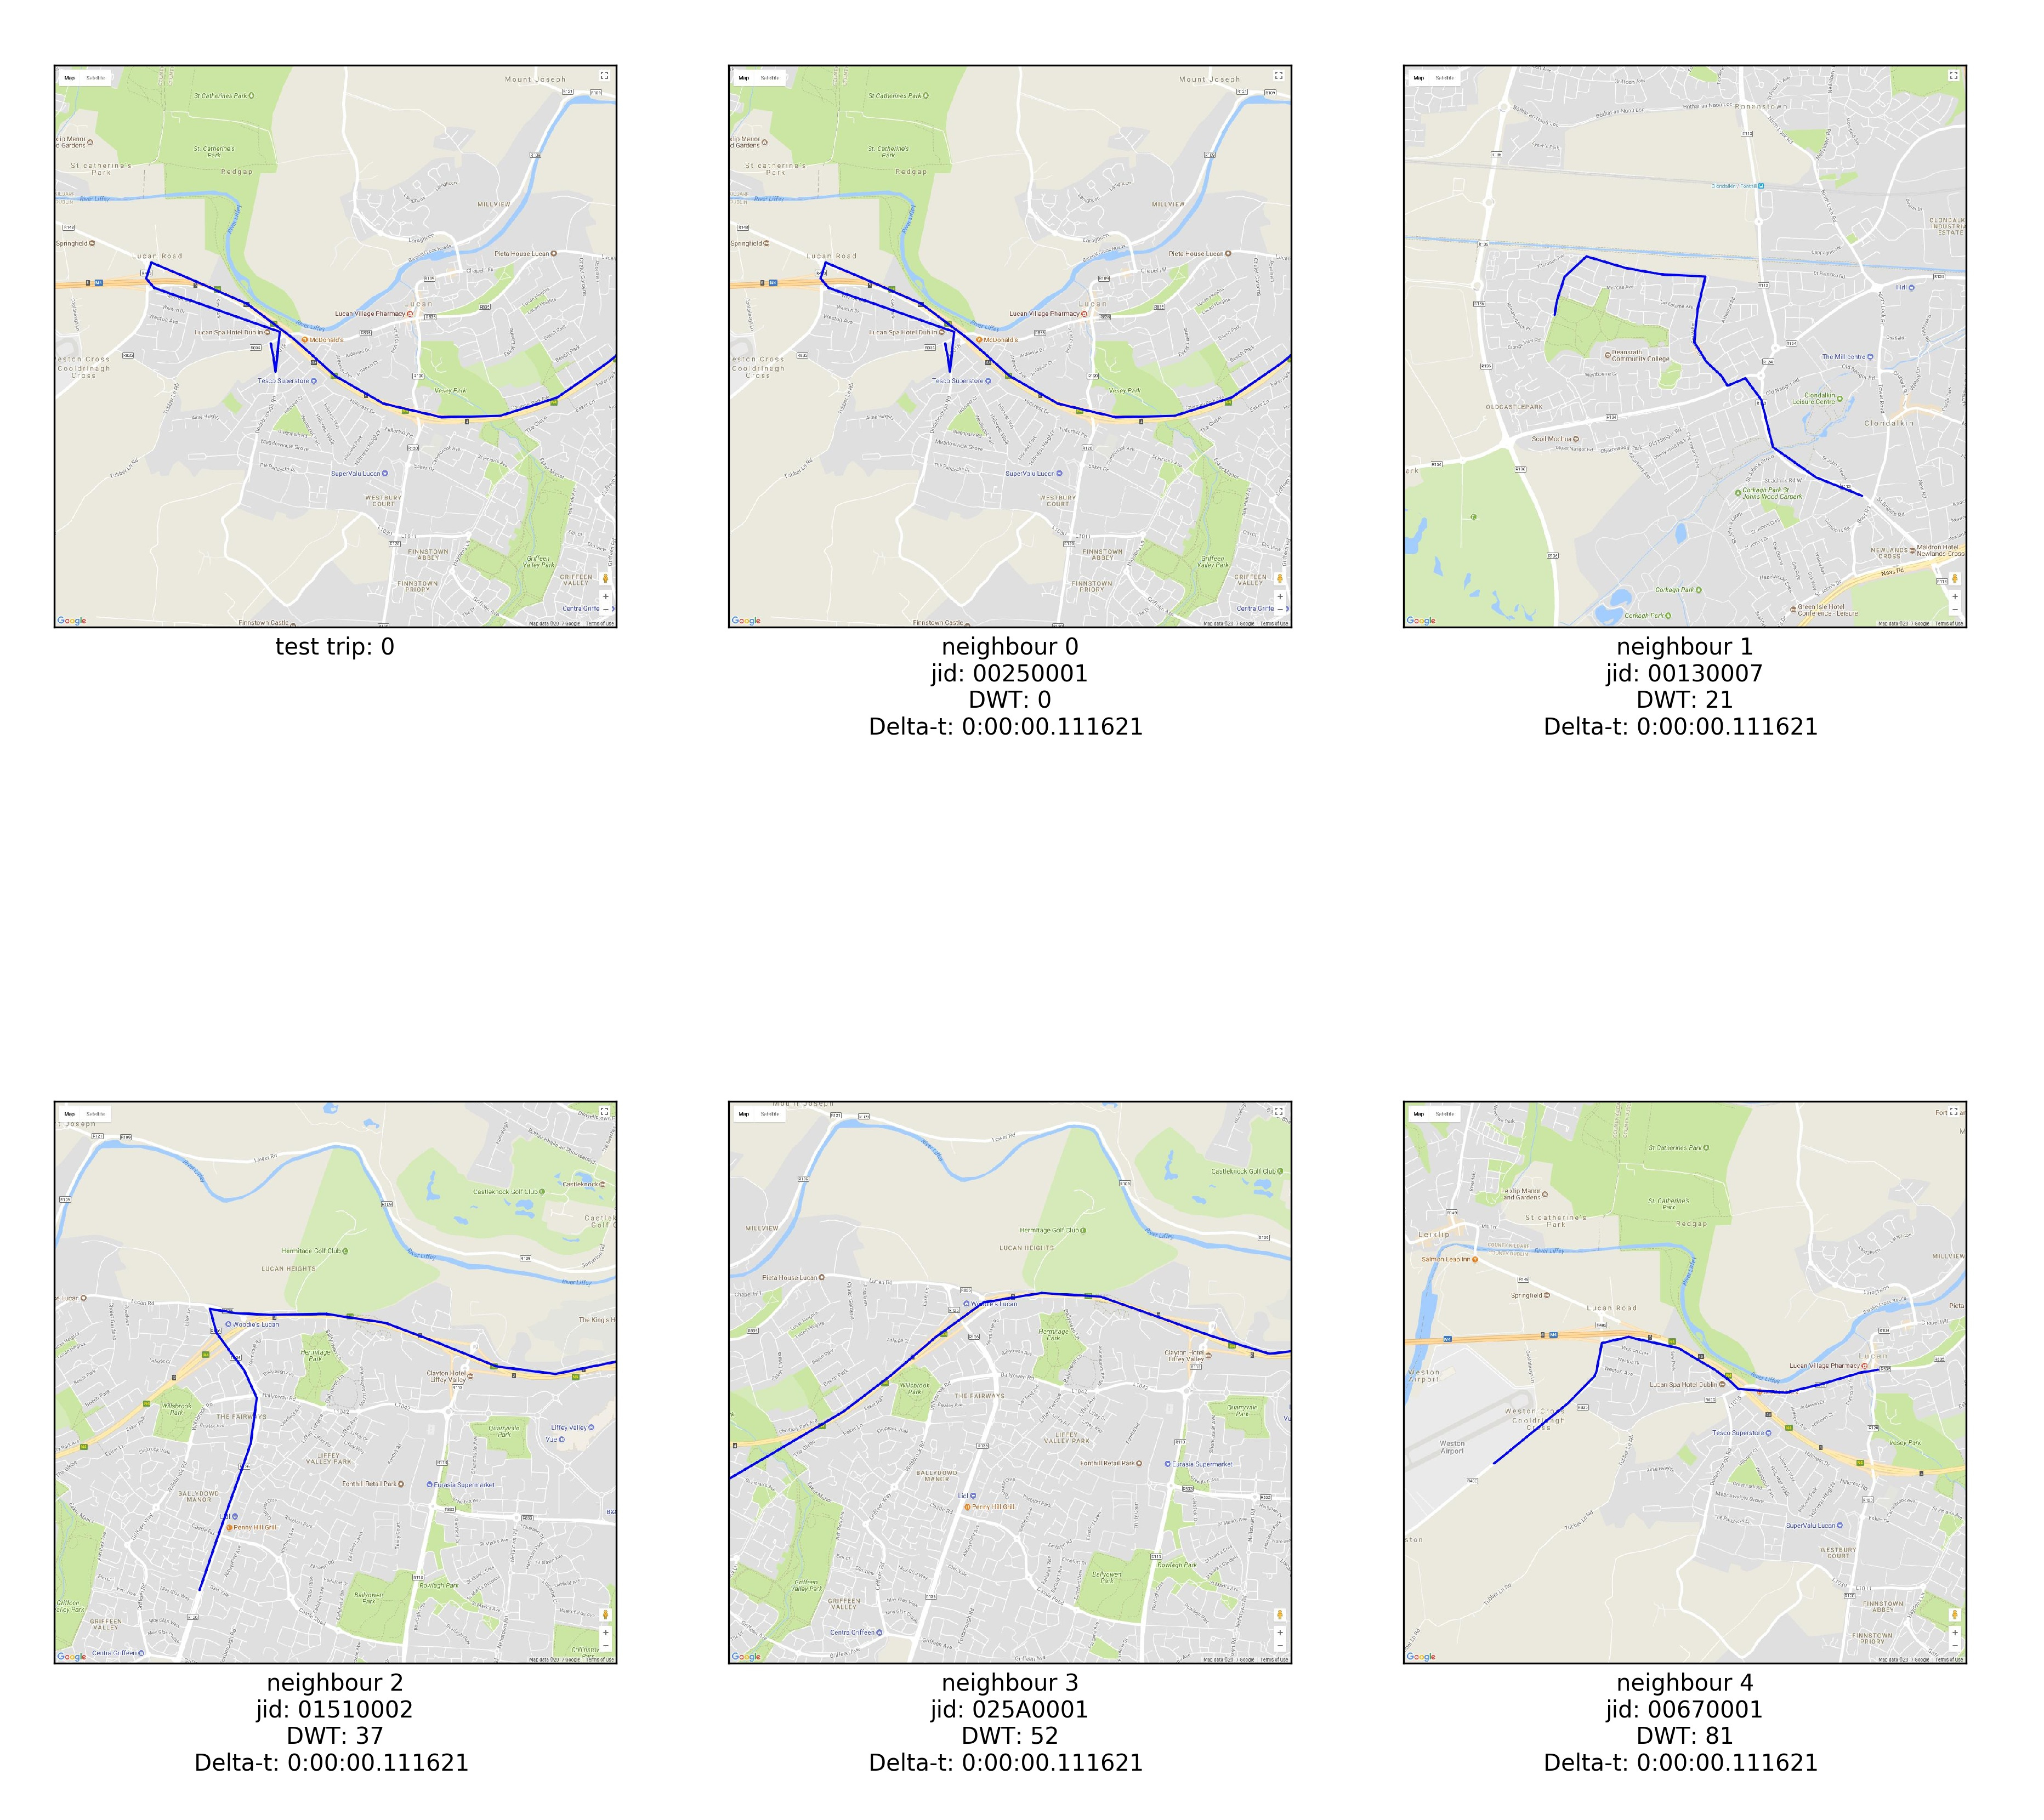
\includegraphics [scale = 0.50] {question2a1example.jpg}
			\caption{Example of nearest neighbours trips visualization}
		\end{center}
	\end{figure} 
	
	\subsection{Nearest Sub-routes (question A2)}
	Following the same logic as above, in the function question\_a2, two dataframes are created for the test and the training dataset using pandas library. The test dataframe is iterated row by row, in order to find the 5 trips from the training dataset which have the longest common subsequence with the specific test trip.
	
	Similarly to the above question, the points are stored as tuples and the required time is calculated using the relevant methods from the utils.py file. To begin with, the method calc\_lcss is called. In this function, the list of lonlat coordinate tuples are given as input. We keep all similar point values and indexes in two lists while iterating the two given lists. The distance between two points is calculated using the method calculate\_lonlat\_distance in the question1.py file. Based on the exercise requirements, two points are considered as equals if their distance is less than 200 metres. Therefore, if the points are equal, and the indexes are the first point of one of the given lists the cell is marked to unit cost and a new similar sequence is started. Otherwise, we continue to an existing similar sequence, increasing by 1 its length, keeping the current cost in the z variable. On the other hand, if points are not equal, then a new subsequence should start, and therefore L[i][j] is set to zero.
	
	Having now found the longest subsequences, we sort the indexes based on the length of the subsequences and we call the update\_current\_maxsubseq in order to update our result comparing previous subsequences. First of all, the new sequences found are iterated, checking if the length of the subsequence list has reached the given number (in our case 5). If there is still space to add the subsequence, then it is added, otherwise we check if the new subsequence is longer from those kept in the list and therefore it should replace it.
	
	Finally, a similar data preprocessing is followed before visualize the data. This time the points are separated so as to show which of them belong to the nearest sub-route and color them with red color. The function for the visualization is the same that was used for the question 2a1 in the utils.py file.
	
	Below, there is an example of the 6 produced maps, showing the nearest sub-routes related to a test trip:
	
	\begin{figure} [H]
		\begin{center}
			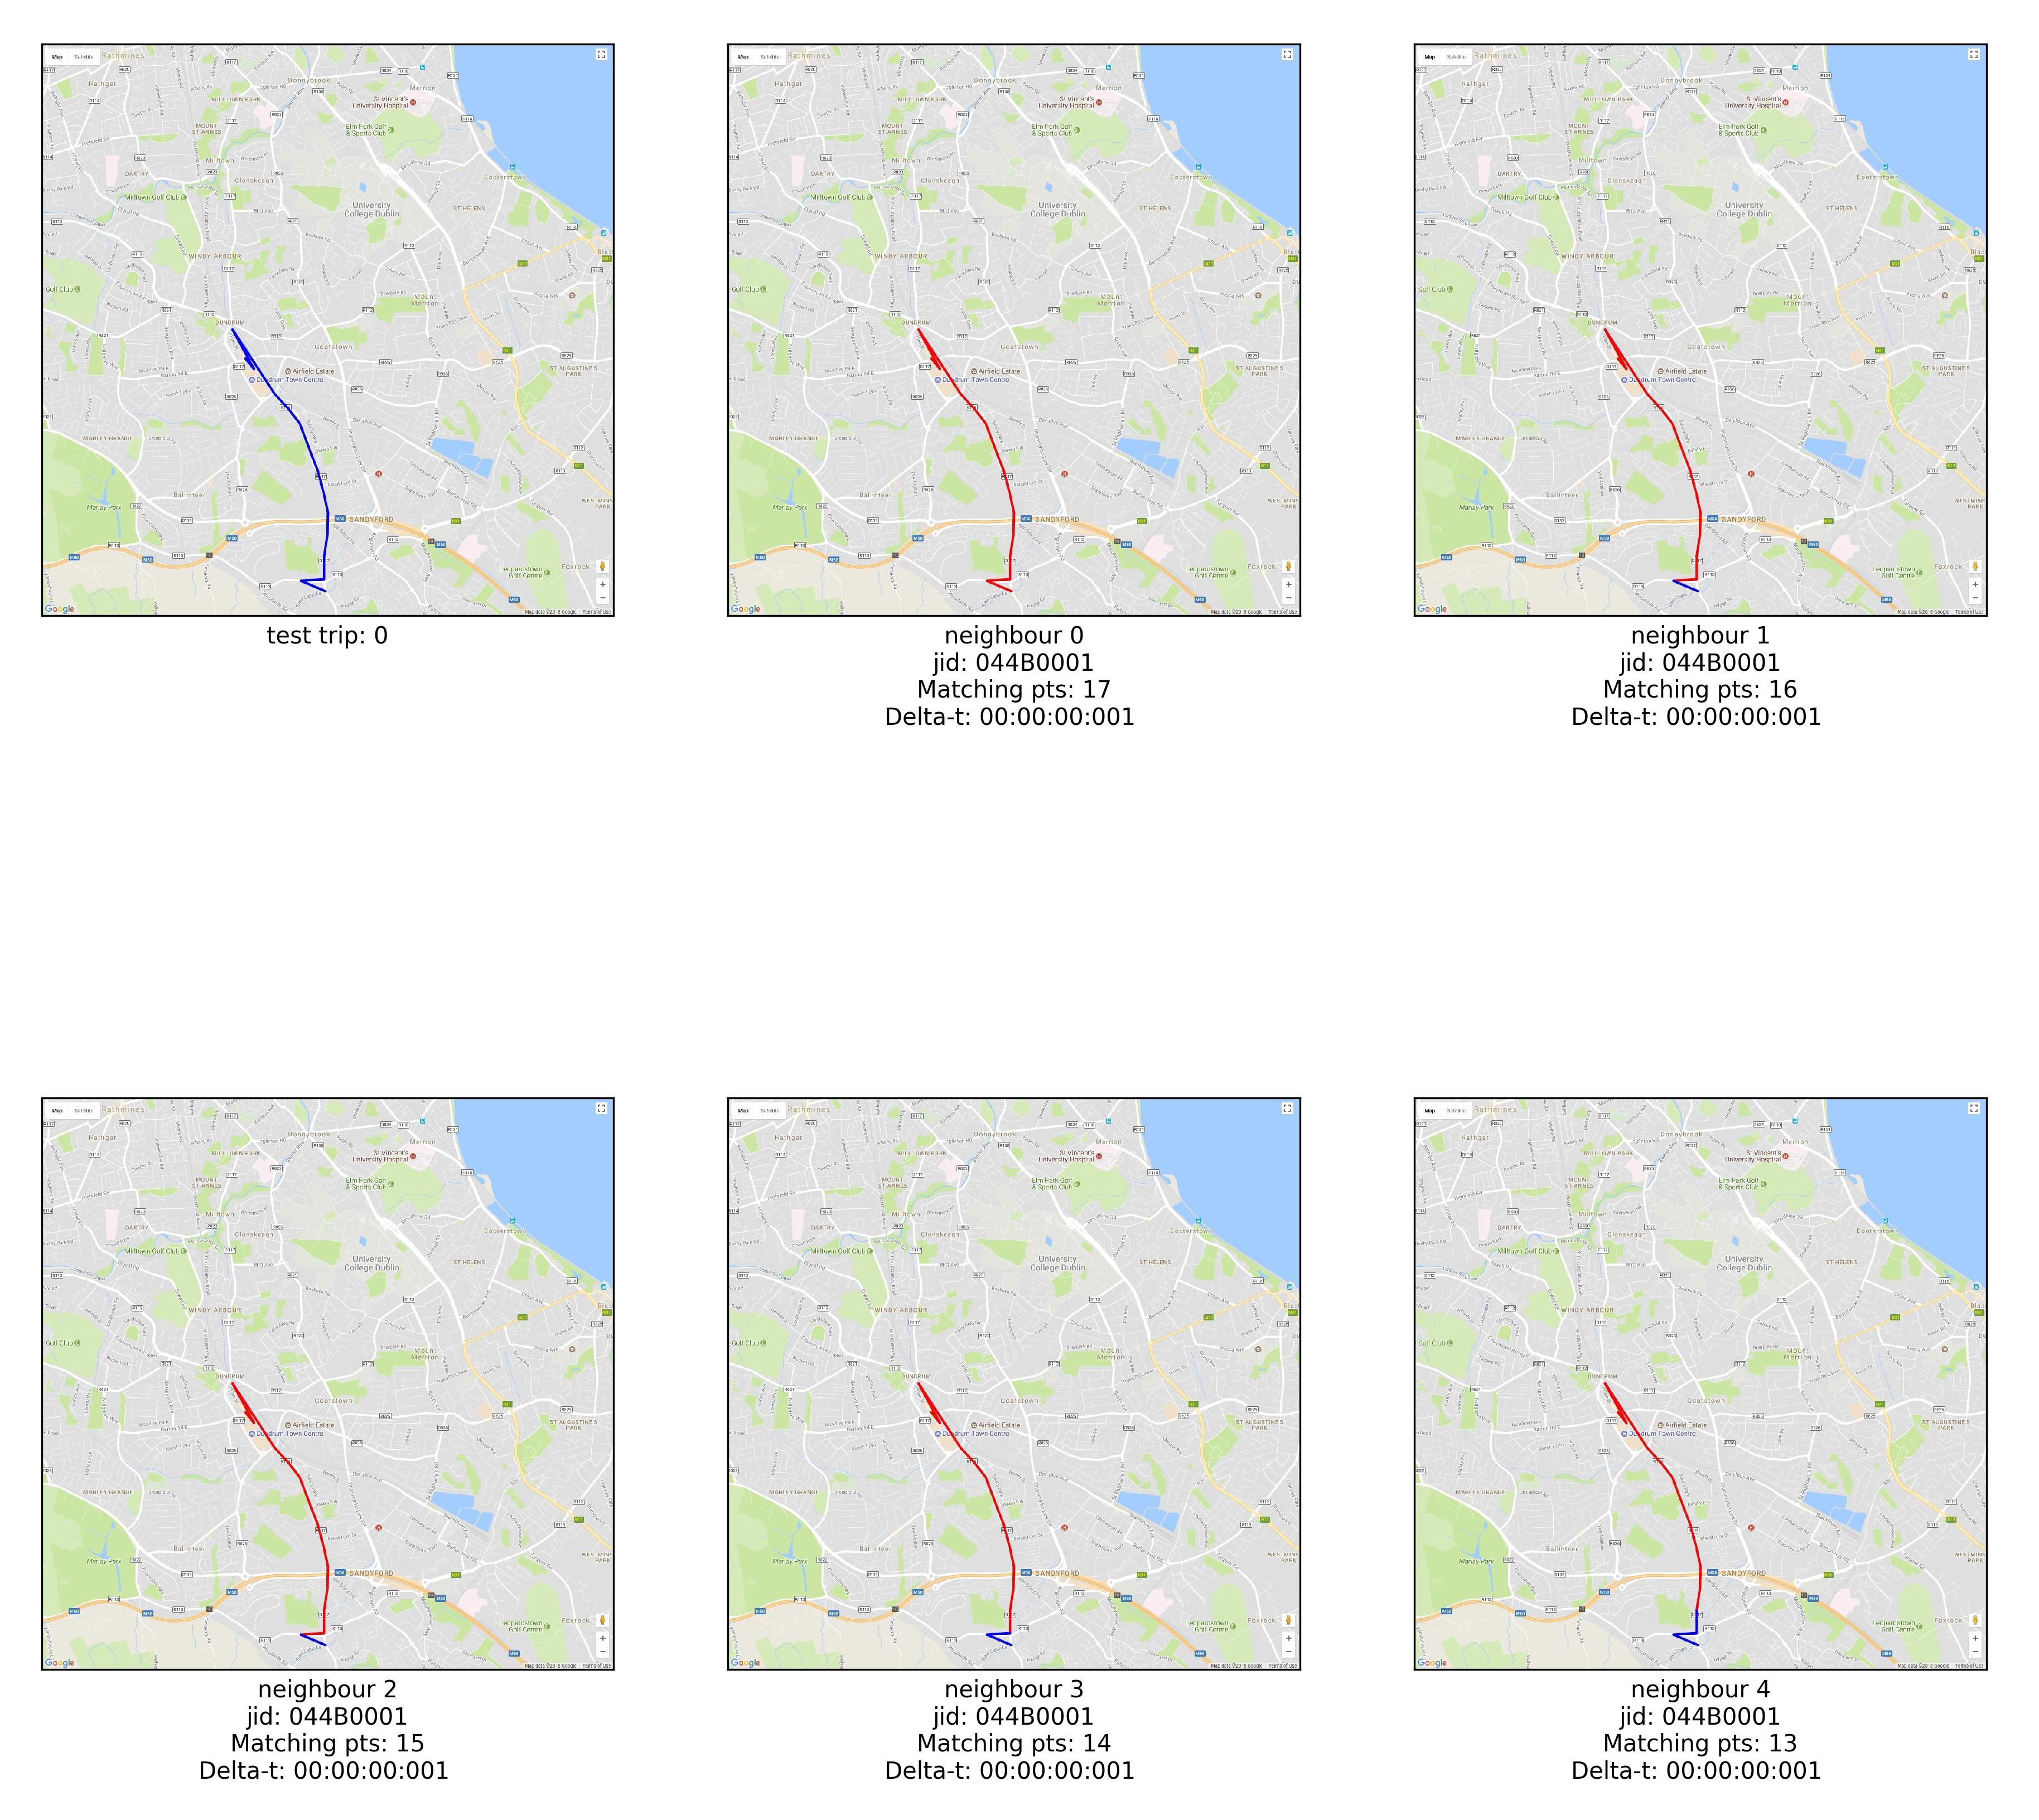
\includegraphics [scale = 0.50] {question2a2example.jpg}
			\caption{Example of nearest sub-routes trips visualization}
		\end{center}
	\end{figure} 
	
	\subsection{Features extraction (question B)}
	The purpose of this task was to export features for classification for the training dataset. In short, a grid should be created and the points of each trip trace should be replaced by a specific square of the grid. The output file where the exported features are stored is the tripFeatures.csv.
	
	In order to be able to draw the grid, it was necessary to find the min and max longitudes and latitudes (function: find\_min\_max\_latlong, file:MapInGridView.py). Having now this information, the next function called is the create\_grid giving as input the number\_of\_cells and the result of the previous method. The distance per cell in the grid is calculated as the difference between the max and the min lat/long divided by the total number of cells. The next step is to create the lines of the rows and the columns and then to provide a name for each cell.
	
	Afterwards, all points in the trip dataframe should be replaced by the cell names that each point corresponds to. This logic is implemented in the method replace\_points. For each row in the dataframe, all coordinates are transformed in tuples format and using the find\_index function a name is mapped to this point. After having replaced all points with their new names, the dataframe is exported in .csv format. In order to be able to easily check the created grid, the method visualize\_grid is implemented so as to plot the grid. 
	
	\subsection{Classification (question C)}
	In the method question\_c, a new dataframe is created from the features file, containing the grid cell names. All functions used in this question are in the file JourneyClassification.py. Before starting the classification, the method preprocess\_data was used in order to get the journey\_id of all trips as numbers and also to remove the letter C from the cell names.
	
	In the requirements of this question it is mentioned to use 10-fold cross validation, therefore the KFold class is used providing the required folds number and then the training dataset is splitted in training and test folds. It worths to be mentioned here, that method asarrays from numpy was used to the, necessary for this question, lists. In addition, a list with the names of the three classifiers is created and for each of them, the relevant function is called in order to train the classifier and then count the predictions' accuracy on the test dataset. 
	
	In this question, the scikit learn library was used. Firstly, for the knn classifier the class KNeighborsClassifier was used, and more specifically the fit and predict methods. In order to calculate the accuracy of the classifiers we have used the accuracy\_score method (this result is return from each classification function in the JourneyClassification.py), but also the classification\_report in order to print the precision and recall values for each prediction of the classifier. The same logic is followed for the other two classifiers(logistic regression and random forest). What should be mentioned, though, is that the LogisticRegression class implements the predict\_proba method, which returns a list with probabilities and argmax from numpy was used in order to determine the result with the max probability.
	
	\subsubsection{Beat ​ ​the ​ ​Benchmark}
	
	\newpage
	\addcontentsline{toc}{section}{References}
	\begin{thebibliography}{30}
		\bibitem{knn}SciKit Learn: Nearest Neighbors \\
		 \url{http://scikit-learn.org/stable/modules/neighbors.html}
		 \bibitem{logreg} SciKit Learn: Logistic Regression \\
		 \url{http://scikit-learn.org/stable/modules/linear_model.html#logistic-regression}
		 \bibitem{ranfor} SciKit Learn: Random Forest \\
		 \url{http://scikit-learn.org/stable/modules/generated/sklearn.ensemble.RandomForestClassifier.html#sklearn.ensemble.RandomForestClassifier}
		 \bibitem{accuracy} SciKit Learn: Accuracy \\
		 \url{http://scikit-learn.org/stable/modules/generated/sklearn.metrics.accuracy_score.html#sklearn.metrics.accuracy_score}
		 \bibitem{knn2}A Complete Guide to K-Nearest-Neighbors with Applications in Python and R \\
		 \url{https://kevinzakka.github.io/2016/07/13/k-nearest-neighbor/}
		 \bibitem{dwt} Dynamic time warping \\
		 \url{https://en.wikipedia.org/wiki/Dynamic_time_warping}
		 \bibitem{lcss} Longest common subsequence problem \\
		 \url{https://en.wikipedia.org/wiki/Longest_common_subsequence_problem}
		 \bibitem{report} SciKit Learn: Classification report \\
		 \url{http://scikit-learn.org/stable/modules/generated/sklearn.metrics.classification_report.html}
		 \bibitem{threads} ThreadPool \\
		 \url{https://stackoverflow.com/questions/8533318/multiprocessing-pool-when-to-use-apply-apply-async-or-map}
    \end{thebibliography}
	
\end{document}
